\documentclass{ctexart}
\usepackage[table]{xcolor}
\usepackage{template_by_mny}
\usepackage{float} 
\usepackage{listings}
\usepackage[figuresright]{rotating}
\lstset{basicstyle=\ttfamily, breaklines=true, frame=single}

\title{光谱仪教学实验报告}
\class{物理 32/物理 31}
\name{冯家琦/周方远}
\id{2023011338/2023011263}

\begin{document}
\maketitle

\begin{abstract}
本报告旨在描述和分析使用EDU-3D1/M偏振和3D影院技术套件进行的3D显示技术实验。实验涉及了3D技术的基本原理、实验仪器的安装与调整、实验步骤的执行以及实验结果的思考和总结。
\end{abstract}

\section{实验原理}
3D显示技术基于将两幅从不同视角捕获的图像分别送入观察者的双眼,从而在大脑中形成深度感知。本实验主要探讨了线性偏振3D技术和RealD方法,后者使用圆偏振光以避免头部倾斜对3D效果的影响。

\section{实验仪器及安装}
\subsection{实验仪器}
\begin{itemize}
    \item EDU-3D1/M偏振和3D影院技术套件
    \item 激光模块
    \item 线性偏振片和四分之一波片(λ/4 plates)
    \item 3D眼镜
    \item 投影屏幕
    \item 光源和滤光片
\end{itemize}
\subsection{仪器安装}
根据EDU-3D1/M套件用户手册,首先安装了铝制面包板和相关的底座、支架。然后,按照说明书,安装了光源、滤光片、偏振片、四分之一波片和3D眼镜的支架。最后,确保了所有组件的对齐和调整,以便进行3D投影实验。

\section{实验步骤}
\subsection{Exercise 1: 应力引起的双折射}

\subsection{Exercise 2: 创建立体图像}
使用相机从两个不同的视角拍摄物体的照片,然后使用免费软件“Anaglyph Maker”将这些照片合成为一幅立体图像。

\subsection{Exercise 3: 红青3D投影}
\begin{enumerate}
    \item 将光源并排设置并向彼此轻微倾斜。
    \item 将幻灯片放置在光源前,确保没有光线穿过幻灯片边缘。
    \item 将红青3D眼镜的一半颜色滤镜分别插入幻灯片后的支架中。
    \item 调整透镜位置,确保图像在屏幕上清晰且重叠。
    \item 佩戴红青3D眼镜观察图像。
\end{enumerate}

\subsection{Exercise 4: 线性偏振3D投影}
\begin{enumerate}
    \item 首先,将偏振片对准所使用的3D眼镜。
    \item 将光源并排设置并向彼此轻微倾斜。
    \item 将幻灯片放置在光源前,确保没有光线穿过幻灯片边缘。
    \item 调整透镜位置,确保图像在屏幕上清晰且重叠。
    \item 在每个光路中添加偏振片,确保没有图像部分被切断。
    \item 进行微调,直到佩戴3D眼镜时获得深度感。
\end{enumerate}

\subsection{Exercise 5: 3D眼镜的构造}
\begin{enumerate}
    \item 将3D眼镜放在线性偏振光源前,旋转眼镜以观察光线透过情况。
    \item 通过旋转眼镜,找到使透射光几乎降至零的特定位置。
\end{enumerate}
可以看到,3D眼镜的两个镜片表现的差异明显,它们分别是线性偏振片和四分之一波片。

\subsection{Exercise 6: 反射光的相位移动}
\begin{enumerate}
    \item 戴上RealD 3D眼镜,站在镜子前,轮流闭上每只眼睛
\end{enumerate}
\begin{figure}[H]
    \centering
    \includegraphics[width=0.5\textwidth]{pictures/3D眼镜.jpg}
    \caption{RealD 3D眼镜的工作原理}
\end{figure}
可以看到,左眼经过四分之一波片后,光线的相位发生了90°的移动,而右眼则没有。因此,右眼在镜面反射后,光线能够正常穿过眼镜,而左眼则无法看到反射光,是一团漆黑如图所示。
\subsection{Exercise 7: 确定眼镜中偏振片的方向}
\begin{enumerate}
    \item 通过将偏振片放置在眼镜后面并照射偏振光,通过旋转偏振片找到角度使得镜片不透光。
    \item 旋转90°,偏振片就位于最大透光位置。
\end{enumerate}

\subsection{Exercise 8: 使用RealD方法设置3D投影}
\begin{enumerate}
    \item \textbf{调整线性滤波器:}首先,需要将实验装置中的偏振片与3D眼镜中的偏振片对齐。使用激光作为辅助工具,将激光通过眼镜,然后线性偏振片放置在眼镜后面,旋转偏振片直到屏幕上没有光照射,确保眼镜直立于支架上。

    \item \textbf{设置幻灯片、光源和透镜:}将屏幕放置在观看图像的位置。将光源稍微相互对准,并大致指向屏幕上的同一点。在光源前放置幻灯片,确保幻灯片的尺寸适合整个光锥通过。调整光源和透镜的位置,使得图像在屏幕上清晰且重叠。

    \item \textbf{定位偏振片和调整波片和滤光片:}在光路中放置每个光源/透镜的偏振片和λ/4波片。调整λ/4波片,戴上RealD眼镜,关闭左眼并旋转右侧的λ/4波片,直到屏幕上的图像大部分变暗。对另一只眼睛和λ/4波片重复此过程。

    \item \textbf{最终调整:}在前面的部分中,每个偏振片和λ/4波片已经被正确调整。现在,必须将图像叠加,以便为观察者创建3D效果。通过轻微调整幻灯片的位置来改变屏幕上图像的偏移,观察屏幕上的深度感如何变化,并持续调整直到3D效果最佳。
\end{enumerate}

通过上述步骤,可以成功设置RealD方法的3D投影,即使头部轻微倾斜,3D效果也能保持稳定。
\begin{figure}[H]
    \centering
    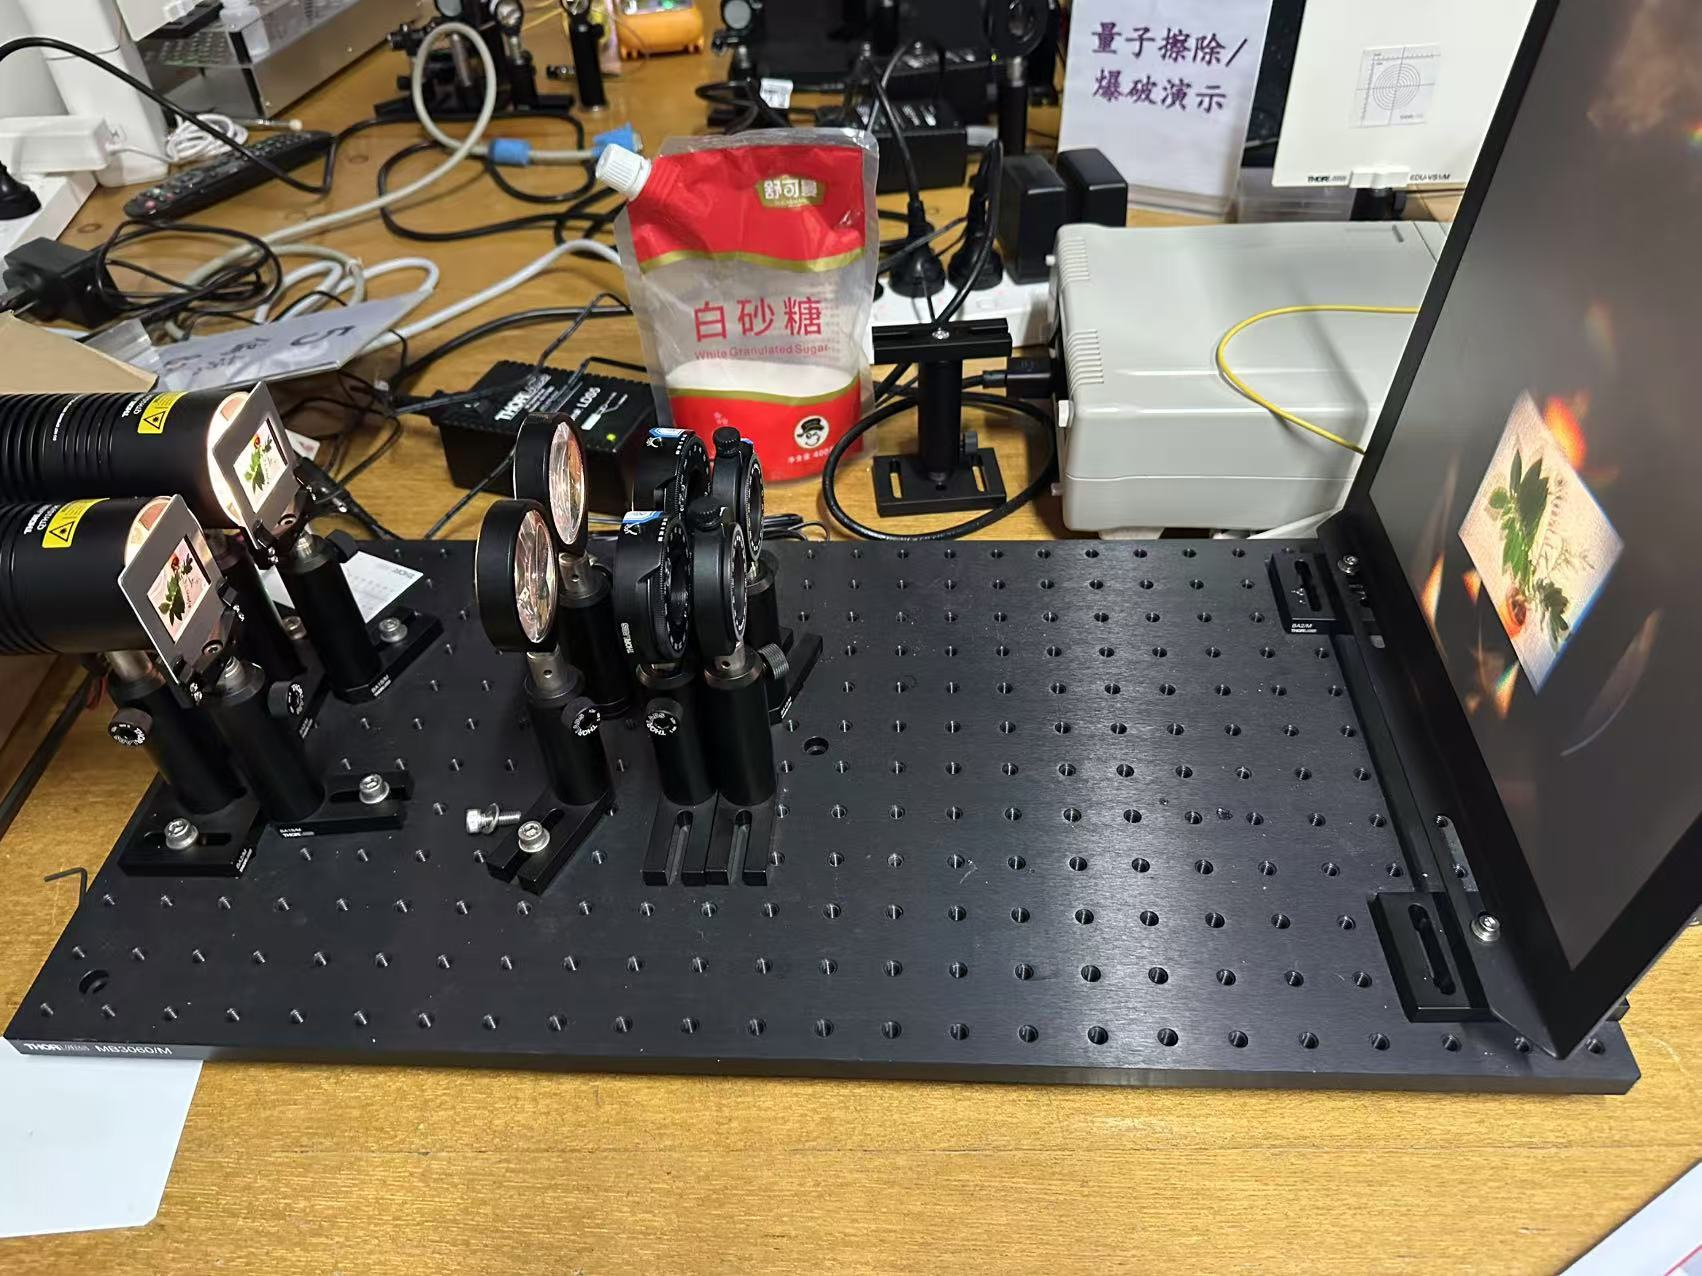
\includegraphics[width=0.5\textwidth]{pictures/微信图片_20241212140323.jpg}
    \caption{RealD 3D技术}
\end{figure}

\section{实验思考}
\begin{itemize}
    \item 讨论了不同3D技术(线性偏振和RealD方法)的优缺点。
    \item 分析了头部倾斜对3D效果的影响,尤其是在使用RealD方法时。
    \item 探讨了如何通过调整图像偏移来优化3D效果。
\end{itemize}

\section{总结}
\begin{itemize}
    \item 实验成功展示了3D显示技术的基本原理和实际操作。
    \item 通过实验,我们深入理解了3D效果是如何通过控制光线的偏振和相位来实现的。
    \item 实验中遇到的问题和解决方案,如对齐偏振片和优化3D效果的方法,都被详细记录和分析。
\end{itemize}

\end{document}